\chapter{Concept - Learning from Data}
\label{chapter:learningFromData}

The following exercises are logic-based, combinatorial puzzles. The idea is that pupils need to conclude the solution by a partially completed grid.

\section{Row of Trees}
\label{section:treeRow}

\subsection{Exercises}
The row of trees is a one dimensional grid i.e a row either of size three or four. In every row there is exactly one tree of every height between one and three (figure \ref{fig:trees_3}), respectively four (figure \ref{fig:trees_4}). At both ends of the row, the amount of visible trees from this end of the row is given and they will be referred to as view slots from now on.

\begin{figure} 
    \centering
    
\includegraphics[width=0.4 \columnwidth]{figures/trees_3.png}
    \caption{Trees from height one to three} 
    \label{fig:trees_3} 
\end{figure}

\begin{figure} 
    \centering
    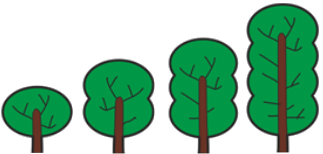
\includegraphics[width=0.4 \columnwidth]{figures/trees_4.png}
    \caption{Trees from height one to four} 
    \label{fig:trees_4} 
\end{figure}

\begin{example}
    An example of a Row of Trees with size three is shown in figure \ref{fig:tree_row_example_exercise}
\end{example}

\begin{figure} 
    \centering
    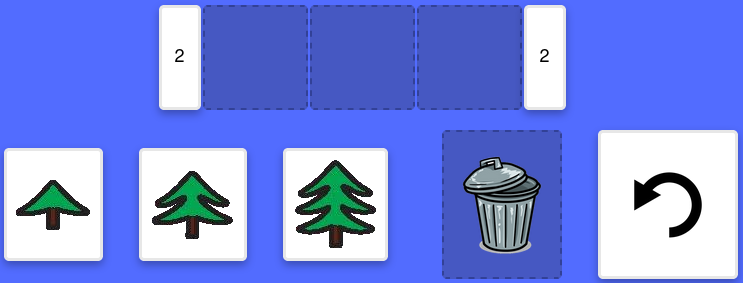
\includegraphics[width=0.8 \columnwidth]{figures/tree_row_example_exercise.png}
    \caption{Row of tree exercise} 
    \label{fig:tree_row_example_exercise} 
\end{figure}

Pupils are given an empty row and two view slots for both ends of the row and they need to place exactly one tree of every height such the row is complete and the aforementioned rules are met.

\begin{example}
    Consider a row of size three. If both view slots have the value $2$, then one possible solution to the puzzle is shown in figure \ref{fig:tree_row_visible_tree}.
\end{example}

\begin{figure} 
    \centering
    
\includegraphics[width=0.8 \columnwidth]{figures/tree_row_example.png}
    \caption{Visualization of the puzzle solution from the tree row example} 
    \label{fig:tree_row_visible_tree} 
\end{figure}

\subsection{Implementation}

The \code{Row.vue} component is implemented to work with any row size. However, since only images of trees for a row size of three and four are present, it makes only sense to use it for those row sizes.

Every number between one and the row size is used as values i.e. for a row size of three, the numbers $1$, $2$ and $3$ are used. Every exercise case is a permutation of these values. Hence the approach is to generate an array with these values, shuffle the array and calculate the view slots for both ends of the row i.e. the array. Listing \ref{lst:rowGeneration} shows this approach and returns view slot values for both ends in form of a tuple.

%TC:ignore
\begin{lstlisting}[language=TypeScript,caption={Algorithm to generate a row of trees exercise instance of \code{this.size}},label={lst:rowGeneration}]
generate(): [number, number] {
  const values = Array.from({ length: this.size }, (_, i) => i + 1);
  this.shuffle(values);
  return [
    this.getVisibleTrees(values),
    this.getVisibleTrees(values.slice().reverse()),
  ];
}
\end{lstlisting}
%TC:endignore

Interesting functions used in listing \ref{lst:rowGeneration} are \code{shuffle} and \code{getVisibleTrees}. 

Apparently, there exists no built-in function in TypeScript, that shuffles an array. Therefore, a own function needs to be implemented. This is not as easy as it seems since, naive approaches may result in different permutations having different probabilities to appear. An implementation that shuffles an array, where all permutations are approximately equal is given in listing \ref{lst:shuffle} \cite{JavaScriptShuffle}.

\code{getVisibleTrees} calculates the amount of trees visible from one end of the row i.e. the arry. An algorithm for calculating this is given in listing \ref{lst:getVisibleTrees}. To calculate the view slot of the other side, the same function can be used and only the array needs to be reversed as shown in listing \ref{lst:rowGeneration}.

%TC:ignore
\begin{lstlisting}[language=TypeScript,caption={Algorithm to shuffle an array},label={lst:shuffle}]
shuffle(arr: number[]): void {
  for (let i = arr.length; i >= 0; i--) {
    const randomIndex = Math.floor(Math.random() * i);

    const temp = arr[i];
    arr[i] = arr[randomIndex];
    arr[randomIndex] = temp;
  }
}
\end{lstlisting}
%TC:endignore

%TC:ignore
\begin{lstlisting}[language=TypeScript,caption={Algorithm to calculate the amount of visible tree from one end},label={lst:getVisibleTrees}]
getVisibleTrees(values: number[]): number {
  let min = 0;
  let visible = 0;
  for (let i = 0; i < values.length; i++) {
    if (values[i] > min) {
      visible++;
      min = values[i];
    }
  }
  return visible;
}
\end{lstlisting}
%TC:endignore

One may have spotted the use of the custom type \code{row}. This custom type is the internal representation of the row and its definition is given in listing \ref{lst:rowType}. A \code{row} is an array of the custom type \code{rowField} and the field \code{value} saves which tree was placed on this field.

%TC:ignore
\begin{lstlisting}[language=TypeScript,caption={Definition of the custom row and rowField type},label={lst:rowType}]
type rowField = {
  id: number;
  value: number;
};
type row = rowField[];
\end{lstlisting}
%TC:endignore

To determine whether a given solution by a pupils is correct or incorrect, the amount of visible trees from both end is again calculated and compared to the view slots. If both match, then the solution is evaluated as correct (listing \ref{lst:rowGeneration}).

%TC:ignore
\begin{lstlisting}[language=TypeScript,caption={Correctness check of a row of tree exercise solution},label={lst:rowCorrectness}]
isCorrect(): boolean {
    const row = this.values.map((field) => field.value);
    const visibleLeft = this.getVisibleTrees(row);
    const visibleRight = this.getVisibleTrees(row.slice().reverse());
    return !(visibleLeft !== this.leftView || visibleRight !== this.rightView);
}
\end{lstlisting}
%TC:endignore

\section{Tree Sudoku}
\label{section:treeSudoku}

\subsection{Exercises}
Tree Sudoku is similar to the well known traditional Sudoku with the difference that trees of different heights are placed instead of numbers, and for both ends of every row and column the amount of visible trees is stated in view slots. The puzzle follows the same rules as the row of trees and is either of size 3x3 or 4x4.

The Tree Sudoku exercise has three different difficulty levels. The difference between the levels is the amount of initially given information for a Tree Sudoku instance:

\begin{itemize}
    \item \textbf{easy} - no views are given and at least 75\% of the trees are placed
    \item \textbf{medium} - some views are given and at least 50\% of the trees are placed
    \item \textbf{hard} - some views are given and only the minimal amount of information to solve the Tree Sudoku instance is given
\end{itemize}

\begin{example}
    An example of a 3x3 Tree Sudoku is shown in figure \ref{fig:tree_sudoku_example_exercise} (level easy)
\end{example}

\begin{figure} 
    \centering
    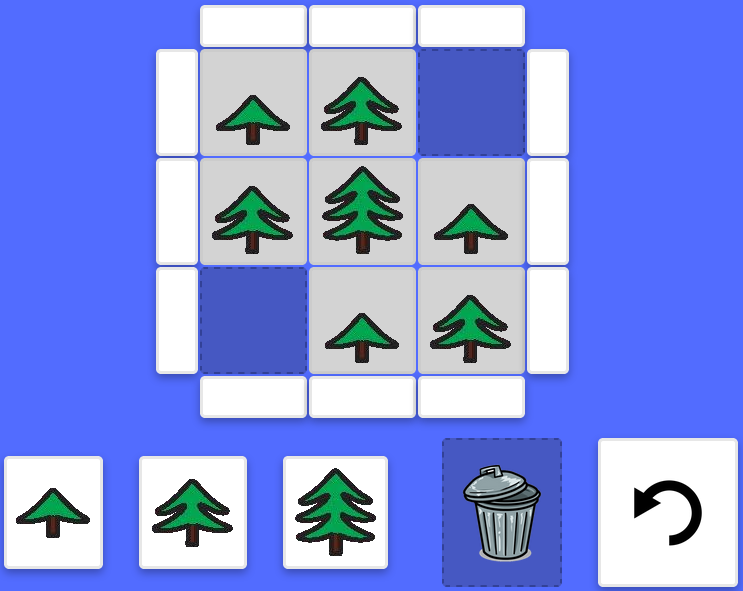
\includegraphics[width=0.6 \columnwidth]{figures/tree_sudoku_example_exercise.png}
    \caption{Tree Sudoku exercise} 
    \label{fig:tree_sudoku_example_exercise} 
\end{figure}

\subsection{Implementation}

The \code{Sudoku.vue} component is implement in a way such that it works with different sizes. In general, a similar approach for the Tree Sudoku exercise is taken like for the \nameref{section:treeRow} exercise. Again, some custom types are used: \code{sudoku} and \code{sudokuField} (listing \ref{lst:sudokuType}). The major difference between these two exercises is that the Tree Sudoku is two-dimensional. Therefore a two-dimensional array is used for the internal representation of the Tree Sudoku grid. A new field used in the \code{sudokuField} compared to the \code{rowField} is \code{locked}. This field indicates that this Tree Sudoku field is part of the initial generation and when the same Tree Sudoku should be restarted, only not locked fields are erased.

%TC:ignore
\begin{lstlisting}[language=TypeScript,caption={Definition of the custom sudoku and sudokuField type},label={lst:sudokuType}]
type sudokuField = {
    id: number;
    value: number;
    locked: boolean;
};

type sudoku = sudokuField[][];
\end{lstlisting}
%TC:endignore

The generation of an instance of the Tree Sudoku exercise is a bit more complicated, since the additional constraints of a Sudoku have to be considered. The approach taken here is to first generate an empty Tree Sudoku. Then in each round, a random tree is placed in a random field or a random value is placed in a random view slot until a solvable configuration is found. 

The most basic operation on a Tree Sudoku is to decide whether it is valid or invalid i.e whether in each row and column every tree height does appear exactly once and whether the views match the placed trees.
The same implementation is used to validate a Tree Sudoku during the generation and when pupils want to check their solution. Empty fields during the generation are allowed, but they are not in a solution of a pupil. Therefore, the validity check takes an additional argument to distinguish between those two cases: \code{complete}.
For both ends of each row and column the amount of visible trees is calculated and if these values match view slots the instance is evaluated as valid. The algorithm to check the validity can be found in listing \ref{lst:sudokuValidation}.

%TC:ignore
\begin{lstlisting}[language=TypeScript,caption={Validation algorithm for a Tree Sudoku instance},label={lst:sudokuValidation}]
isValid(values: sudoku, views: number[][], complete: boolean): boolean {
  for (let i = 0; i < values.length; i++) {
    const rowSeen = new Set<number>();
    const colSeen = new Set<number>();
    for (let j = 0; j < values[i].length; j++) {
      const traversal: [number, Set<number>][] = [
        [values[i][j].value, rowSeen],
        [values[j][i].value, colSeen],
      ];
      for (let k = 0; k < traversal.length; k++) {
        const [el, seen] = traversal[k];
        if (seen.has(el)) {
          return false;
        } else if (el === 0) {
          if (complete) {
            return false;
          }
          continue;
        } else {
          seen.add(el);
        }
      }
    }

    if (rowSeen.size === this.size) {
      const row = values[i].map((el) => el.value);
      const visible = this.getVisibleTrees(row);
      const visibleRev = this.getVisibleTrees(row.slice().reverse());
      if (
        (views[1][i] !== 0 && views[1][i] !== visible) ||
        (views[2][i] !== 0 && views[2][i] !== visibleRev)
      ) {
        return false;
      }
    }
    if (colSeen.size === this.size) {
      const col: number[] = [];
      for (let k = 0; k < values.length; k++) {
        col[k] = values[k][i].value;
      }
      const visible = this.getVisibleTrees(col);
      const visibleRev = this.getVisibleTrees(col.slice().reverse());
      if (
        (views[0][i] !== 0 && views[0][i] !== visible) ||
        (views[3][i] !== 0 && views[3][i] !== visibleRev)
      ) {
        return false;
      }
    }
  }
  return true;
}
\end{lstlisting}
%TC:endignore

A Tree Sudoku generator needs a Tree Sudoku solver to check whether an instance is actually solvable. Solving a Tree Sudoku means that one needs to repeatedly place trees in fields such that the Tree Sudoku remains valid. The Tree Sudoku generator requires to know how many solutions a Tree Sudoku has to use it as a stopping criterion. Hence, the solving algorithm shown in listing \ref{lst:sudokuSolver} additionally counts how many solutions exist and returns it.

%TC:ignore
\begin{lstlisting}[language=TypeScript,caption={Solving algorithm for a Tree Sudoku instance},label={lst:sudokuSolver}]
solve(values: sudoku, views: number[][]): number {
  const [complete, emptyValueSlotRow, emptyValueSlotCol] = this.findEmptySlot(
    values.map((row) => row.map((col) => col.value))
  );
  if (complete) {
    this.valuesSolution = JSON.parse(JSON.stringify(values)) as sudoku; // deep copy
    return 1;
  }

  let solutions = 0;
  for (let i = 1; i <= this.size; i++) {
    values[emptyValueSlotRow][emptyValueSlotCol].value = i;
    if (this.isValid(values, views, false)) {
      solutions += this.solve(values, views);
      if (solutions > 1) {
        break;
      }
    }
  }
  values[emptyValueSlotRow][emptyValueSlotCol].value = 0;
  return solutions;
}
\end{lstlisting}
%TC:endignore

Generating a Tree Sudoku requires to first independently find any empty field and any empty end of a row or column and then to pick with a probability of 0.5 either the empty field or the empty end of a row or column. Next, a random number is put in the picked field. After that, the validity of the Tree Sudoku is checked and if it is valid, the amount of possible solutions for the Tree Sudoku is calculated. If no solution is found, a different number has to be tried. If more than one solutions are found, we start all over again by choosing a random empty field or empty end of a row or column. If the Tree Sudoku has exactly one solution, then the Tree Sudoku is uniquely solvable and the algorithm stops. An implementation of the here mentioned algorithm can be found in listing \ref{lst:sudokuGenerator}.

%TC:ignore
\begin{lstlisting}[language=TypeScript,caption={Generation algorithm for a Tree Sudoku instance},label={lst:sudokuGenerator}]
generate(values: sudoku, views: number[][]): [sudoku, number[][]] {
  const [
    valuesComplete,
    emptyValueSlotRow,
    emptyValueSlotCol,
  ] = this.findEmptySlot(values.map((row) => row.map((col) => col.value)));
  if (valuesComplete) {
    return [values, views];
  }
  const [
    viewsComplete,
    emptyViewSlotRow,
    emptyViewSlotCol,
  ] = this.findEmptySlot(views);
  if (viewsComplete) {
    return [values, views];
  }

  const numbers: number[] = [];
  for (let i = 0; i < this.size; i++) {
    numbers[i] = i + 1;
  }
  this.shuffle(numbers);
  for (let i = 0; i < numbers.length; i++) {
    if (
      this.randomNumber(1) <= 0.5 ||
      this.LevelsWithNoViews.includes(this.currentDifficultyLevel)
    ) {
      values[emptyValueSlotRow][emptyValueSlotCol].value = numbers[i];
      values[emptyValueSlotRow][emptyValueSlotCol].locked = true;
    } else {
      views[emptyViewSlotRow][emptyViewSlotCol] = numbers[i];
    }
    if (this.isValid(values, views, false)) {
      const solutions = this.solve(values, views);
      if (solutions === 0) {
        values[emptyValueSlotRow][emptyValueSlotCol].value = 0;
        values[emptyValueSlotRow][emptyValueSlotCol].locked = false;
        views[emptyViewSlotRow][emptyViewSlotCol] = 0;
        continue;
      } else if (solutions === 1) {
        return [values, views];
      } else {
        return this.generate(values, views);
      }
    } else {
      values[emptyValueSlotRow][emptyValueSlotCol].value = 0;
      values[emptyValueSlotRow][emptyValueSlotCol].locked = false;
      views[emptyViewSlotRow][emptyViewSlotCol] = 0;
    }
  }
  return [values, views];
}
\end{lstlisting}
%TC:endignore

To fit the requirements of each difficulty level, the generated Tree Sudoku is solved field by field until the difficulty level specific coverage percentage is reached.

To check whether a solution to Tree Sudoku exercise handed in by a pupils, the algorithm from listing \ref{lst:sudokuValidation} can be reused without allowing empty fields.

The algorithm from listing \ref{lst:sudokuValidation} is reused without allowing empty fields, to validate a handed-in solution.
